\documentclass[10pt]{article}
\input{style/coursHeadings}
\input{style/programHeadings}
\input{style/macros_SII}
\input{style/macros_Titres}
\input{style/macros_Frames}

%Si le boolen xp est vrai : compilation pour xabi
%Sinon compilation Damien
\newboolean{xp}
\setboolean{xp}{true}

\newboolean{prof}
\setboolean{prof}{false}

\usepackage[%
    pdftitle={CI3 - CIN -- Torseurs -- TD},
    pdfauthor={Xavier Pessoles},
    colorlinks=true,
    linkcolor=blue,
    citecolor=magenta]{hyperref}

\def\discipline{Sciences Industrielles de l'Ingénieur}
\def\xxtitre{\ifthenelse{\boolean{xp}}{%CI 3 -- CIN : Étude du comportement cinématique des systèmes
}{
Chapitre  -- }}

\def\xxsoustitre{\ifthenelse{\boolean{xp}}{
CI 3 -- CIN : Étude du comportement cinématique des systèmes}{
Partie  -- }}
\def\xxauteur{\ifthenelse{\boolean{xp}}{
\noindent 2013 -- 2014 \\
TDs de Stéphane Genouël}{
Damien \textsc{Iceta} \\ Xavier \textsc{Pessoles}}}

\def\xxpied{\ifthenelse{\boolean{xp}}{
CI 3 : CIN -- TD\\
Ch. 7 : Torseurs -- \ifthenelse{\boolean{prof}}{P}{E}}{
\xxtitre}}

\def\xxcathegorie{\ifthenelse{\boolean{xp}}{
2013 -- 2014 \\
Xavier \textsc{Pessoles}}{
Informatique - Cours}}





%---------------------------------------------------------------------------


\begin{document}

\ifthenelse{\boolean{xp}}{\input{style/enteteXP}}{\input{style/enteteDI}}

\begin{center}
\large{\textsc{Chapitre 6 -- }}
\end{center}

\begin{center}
\textsc{Travaux dirigés}
\end{center}

\normalsize

\begin{flushright}
\textit{D'après ressources de S. Genouël}
\end{flushright}

  \renewcommand{\baselinestretch}{1.2}
%\setlength{\parskip}{2ex plus 0.5ex minus 0.2ex}




\section*{Système de distribution d'un moteur 4 temps}
\setcounter{subparagraph}{0}

 
Le système de distribution automobile permet l’admission du mélange gaz frais (air + carburant) et le 
refoulement des gaz d’échappement lors du cycle 4 temps d’un moteur thermique. 
Le vilebrequin (arbre moteur) entraine en rotation l’arbre à came par l’intermédiaire d’une transmission 
poulie/courroie crantée (courroie de distribution). Le mouvement de rotation continue de l’arbre à cames 1 
est ensuite transformé en un mouvement de translation alternative de l’ensemble poussoir+soupape 2.

\begin{center}
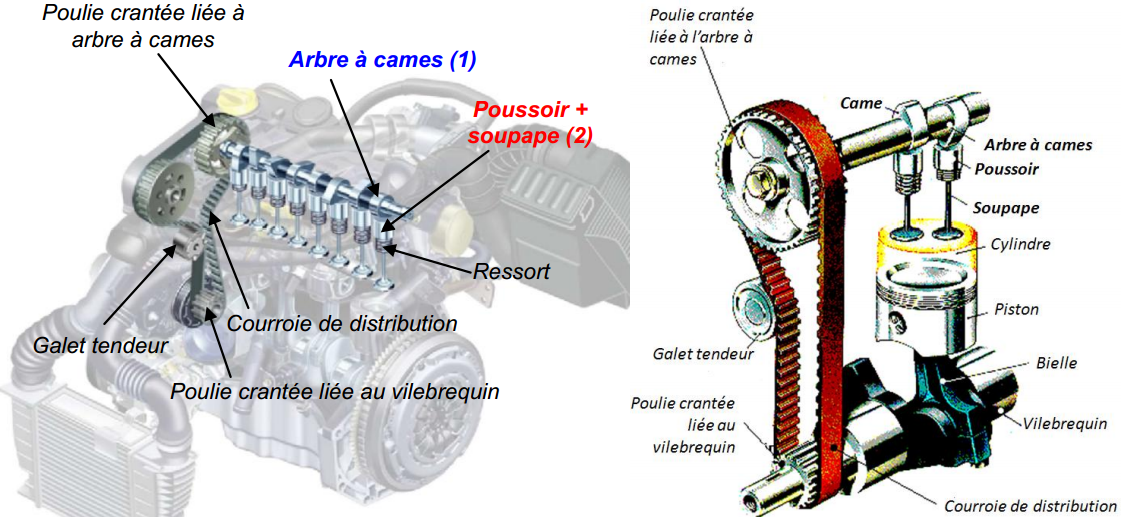
\includegraphics[width=.8\textwidth]{images/fig_01}
\end{center}
On s’intéresse dans la suite, au comportement cinématique de ce dispositif de transformation de mouvement 
par came. Pour simplifier l’étude, on l’assimilera un dispositif de transformation de mouvement par 
excentrique. 


\begin{center}
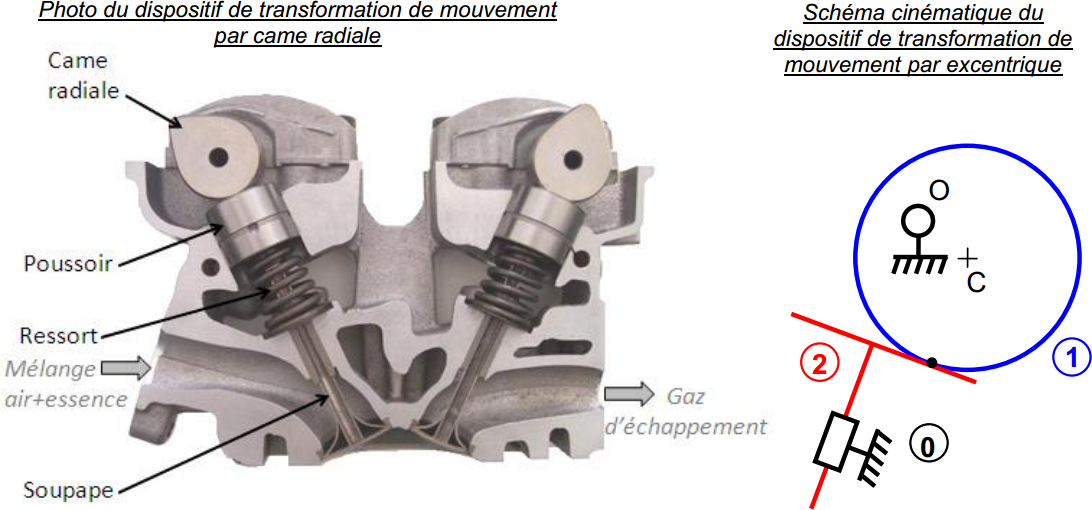
\includegraphics[width=.8\textwidth]{images/fig_02}
\end{center}
\subsubsection*{Constituants et paramétrage}
Le carter 0, de repère associé $\mathcal{R}_0\left( O,\vect{x_0},\vect{y_0},\vect{z_0}\right)$ est considéré comme fixe. 

L’arbre à came 1, de repère associé 
$\mathcal{R}_1\left( O,\vect{x_1},\vect{y_1},\vect{z_1}\right)$, est en mouvement de rotation d’axe $\left(O,\vect{z_0} \right)$ par rapport au carter 0 tel que $\vect{z_0}=\vect{z_1}$ et 
$\left(\vect{x_0},\vect{x_1}\right)=\theta$. La came, représentée par un disque de rayon $R$ et de centre $C$ tel que $\vect{OC}=e\vect{x_1}$, est en contact ponctuel au point $I$ de normale $(I,\vect{z_0})$ avec l’ensemble poussoir+soupape 2. 

L’ensemble poussoir+soupape 2, de repère associé $\mathcal{R}_2\left( A,\vect{x_2},\vect{y_2},\vect{z_2}\right)$, est en mouvement de translation rectiligne de direction 
$\vect{y_0}$ par rapport au carter 0 tel que $\vect{OA}=\lambda \vect{y_0}$.



\begin{center}
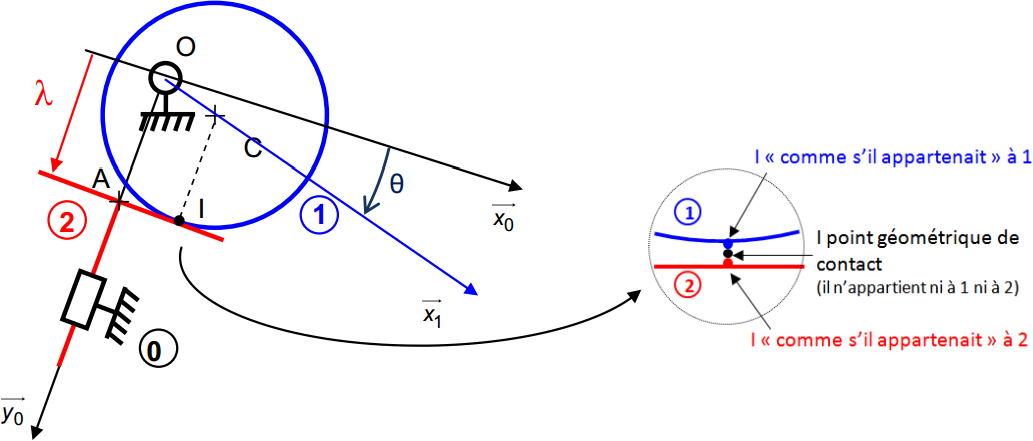
\includegraphics[width=.8\textwidth]{images/fig_03}
\end{center}

\subsection*{Étude géométrique}

\subparagraph{}
\textit{Déterminer les trajectoires $T_{I\in 1/0}$ et $T_{I\in 2/0}$.}
\ifthenelse{\boolean{prof}}{
\begin{corrige}
\end{corrige}}{}



\subparagraph{}
\textit{Déterminer la trajectoire de $I$ (point géométrique de contact) :
\begin{itemize}
\item [$\bullet$] dans $\mathcal{R}_2$;
\item [$\bullet$] dans $\mathcal{R}_1$;
\item [$\bullet$] dans $\mathcal{R}_0$.
 \end{itemize}}
\textit{Rappel : Pour déterminer la trajectoire d’un point géométrique de contact dans un repère 
quelconque, on détermine d'abord son vecteur position dans ce repère. }
\ifthenelse{\boolean{prof}}{
\begin{corrige}
\end{corrige}}{}


\subsection*{Étude cinématique graphique}

\subparagraph{}
\textit{Donner la désignation du vecteur vitesse de glissement de cet exercice. Avec quelle méthode graphique, pourrions-nous déterminer ce vecteur ? }
\ifthenelse{\boolean{prof}}{
\begin{corrige}
\end{corrige}}{}

\subsection*{Étude cinématique analytique}

\subparagraph{}
\textit{Calculer ce vecteur vitesse de glissement.}% selon les 2 méthodes du cours.}
\ifthenelse{\boolean{prof}}{
\begin{corrige}
\end{corrige}}{}


\subparagraph{}
\textit{Préciser les composantes de roulement et de pivotement en $I$.}
\ifthenelse{\boolean{prof}}{
\begin{corrige}
\end{corrige}}{}

\newpage

\section*{Guidage linéaire de systèmes médicaux}
\setcounter{subparagraph}{0}

\begin{minipage}[c]{.7\linewidth}
L’étude suivante porte sur le guidage en translation d’un chariot 
de scanner médical S1 par rapport au bâti de la machine S0. Ce 
guidage est réalisé par deux séries de billes, S2 et S3, qui roulent 
dans des rainures en V. 
\end{minipage}
\begin{minipage}[c]{.25\linewidth}
\begin{center}
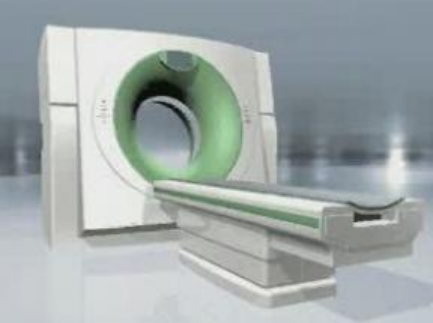
\includegraphics[width=.95\textwidth]{images/fig_04}
\end{center}
\end{minipage}

La figure ci-dessous présente, en coupe, la réalisation technologique de ce guidage. 

\begin{center}
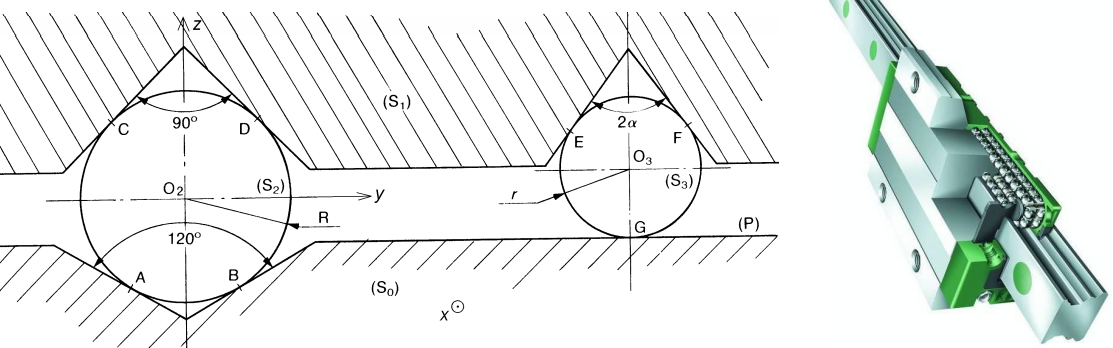
\includegraphics[width=.85\textwidth]{images/fig_05}
\end{center}

Les billes S2 de rayon $R$ roulent sans glisser sur les plans d’une rainure en V d’angle égal à 90\textdegree usinée dans 
S1 et sur les plans d’une autre rainure en V d’angle égal à 120\textdegree usinée dans S0. 
Les billes S3 de rayon $r$ roulent sans glisser sur les plans d’une rainure en V d’angle égal à 
$2\alpha$ usinée dans 
S1 et sur le plan (P) de S0. 

On note $\torseurcin{V}{1}{0}=\torseurl{\vect{0}}{v\vect{x}}{\forall P}$ le torseur cinématique du mouvement du chariot S1 par rapport au bâti S0. 

On pose $\vecto{2}{0} = \omega_{20}\vect{y}$ et $\vecto{3}{0} = \omega_{30}\vect{y}$.

\subparagraph{}
\textit{Traduire les conditions de non glissement. En déduire quelques axes instantanés de rotation.}
\ifthenelse{\boolean{prof}}{
\begin{corrige}
\end{corrige}}{}

\subparagraph{}
\textit{Déterminer $\vectv{C}{2}{0}$ en fonction de $v$, puis $\vectv{E}{3}{0}$ en fonction de $v$. Déterminer $\vectv{C}{2}{0}$ en fonction de $\omega_{20}$, puis $\vectv{E}{3}{0}$ en fonction de $\omega_{30}$. En déduire une relation entre $\omega_{20}$ et $v$, puis une relation entre $\omega_{30}$ et $v$.}
\ifthenelse{\boolean{prof}}{
\begin{corrige}
\end{corrige}}{}

\subparagraph{}
\textit{En déduire les torseurs cinématiques des mouvements de S2/S0 et S3/S0 en fonction de v et 
des caractéristiques géométriques.}
\ifthenelse{\boolean{prof}}{
\begin{corrige}
\end{corrige}}{}

\subparagraph{}
\textit{Préciser les composantes de roulement et de pivotement en $G$ et $B$.}
\ifthenelse{\boolean{prof}}{
\begin{corrige}
\end{corrige}}{}

\subparagraph{}
\textit{Déterminer les vecteurs vitesses des centres des billes dans leur mouvement par rapport au bâti S0 : $\vectv{O_2}{2}{0}$ et $\vectv{O_3}{3}{0}$.}
\ifthenelse{\boolean{prof}}{
\begin{corrige}
\end{corrige}}{}

\subparagraph{}
\textit{Déterminer $\alpha$ pour que ces vecteurs vitesses soient identiques. }
\ifthenelse{\boolean{prof}}{
\begin{corrige}
\end{corrige}}{}



\newpage

\section*{Banc de tests pneumatiques}
\setcounter{subparagraph}{0}


\begin{minipage}[c]{.7\linewidth}
Un banc de tests d’usure de pneumatiques est représenté ci-contre. 
 
Un ensemble pneumatique + jante 2, entrainé en rotation par rapport 
au bras 3 à l’aide d’un moto-réducteur, roule sur un plateau tournant 
1. 
Le bras 3 est le plateau tournant 1 sont entrainé en rotation par rapport 
aux bâti 0 à l’aide de deux autres moto-réducteurs.
\end{minipage}
\begin{minipage}[c]{.25\linewidth}
\begin{center}
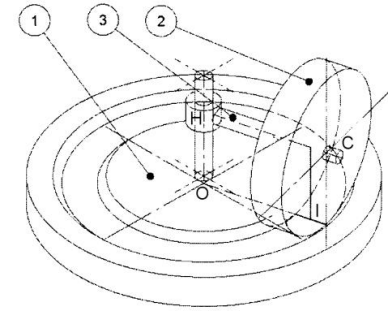
\includegraphics[width=\textwidth]{images/fig_06}
\end{center}
\end{minipage}




\begin{minipage}[c]{.45\linewidth}
Schéma simplifié : on considère la roue 2 comme un disque. 
\begin{center}
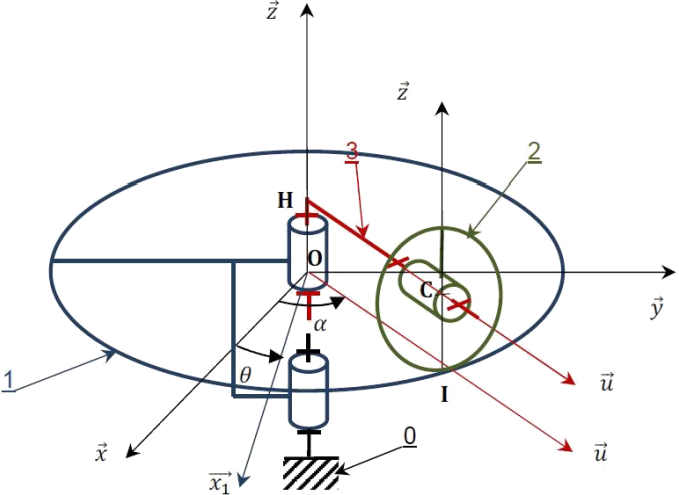
\includegraphics[width=\textwidth]{images/fig_07}
\end{center}
\end{minipage} \hfill
\begin{minipage}[c]{.53\linewidth}

Le paramétrage est le suivant : 
\begin{itemize}
\item $\mathcal{R}_0\left( O,\vect{x},\vect{y},\vect{z}\right)$  est associé au bâti 0 considéré comme fixe;
\item le plateau tournant 1, de repère associé $\mathcal{R}_1\left( O,\vect{x_1},\vect{y_1},\vect{z_1}\right)$, est en mouvement de rotation d’axe $\left(O,\vect{z}\right)$ par rapport au bâti 0 tel que $\vect{z}=\vect{z_1}$ et $\theta=\left(\vect{x},\vect{x_1}\right)$;
\item le bras 3, de repère associé $\mathcal{R}_3\left( H,\vect{u},\vect{v},\vect{w}\right)$ est en mouvement de rotation d’axe $\left(O,\vect{z}\right)$ par rapport au bâti 0 tel que $\vect{z}=\vect{w}$ et $\alpha = \left(\vect{x},\vect{u}\right)$;
\item l’ensemble pneumatique + jante 2, de repère associé, $\mathcal{R}_2\left( O,\vect{x_2},\vect{y_2},\vect{z_2}\right)$ est en mouvement de rotation d’axe $\left(H,\vect{u}\right)$ par rapport au bras 3 tel que $\vect{u}=\vect{x_2}$ et $\beta = \left(\vect{z},\vect{z_2}\right)$. On pose $\vect{HC}=d\vect{u}$ (d est constante). Le pneumatique de rayon $r$ est en contact au point $I$ avec le plateau 1. 
\end{itemize}
\end{minipage}

\begin{Objectif}
Déterminer la relation entre les vitesses de rotation des 3 actionneurs permettant de reproduire 
des conditions de roulement sans glissement d’un pneumatique sur une route. 
\end{Objectif}
%\subparagraph{}
%\textit{Quelle condition le vecteur $\vectv{I}{2}{1}$ doit-il satisfaire pour assurer le maintien du contact entre 
%les solides 2 et 1 au point I. }
%\ifthenelse{\boolean{prof}}{
%\begin{corrige}
%\end{corrige}}{}

\subparagraph{}
\textit{Quelle condition le vecteur $\vectv{I}{2}{1}$ doit-il satisfaire pour assurer le maintien du contact entre les solides 2 et 1 en $I$.}

\subparagraph{}
\textit{Déterminer $\vectv{I}{2}{1}$.}
\ifthenelse{\boolean{prof}}{
\begin{corrige}
\end{corrige}}{}

\subparagraph{}
\textit{Déterminer le vecteur vitesse de glissement au point $I$.}% selon 2 méthodes différentes.}
\ifthenelse{\boolean{prof}}{
\begin{corrige}
\end{corrige}}{}

\subparagraph{}
\textit{Dans les conditions de roulement sans glissement en $I$, en déduire la relation entre $\dot{\theta}$, $\dot{\alpha}$, $\dot{\beta}$ (vitesses de rotation des 3 actionneurs) et les dimensions du système.}
\ifthenelse{\boolean{prof}}{
\begin{corrige}
\end{corrige}}{}

\subparagraph{}
\textit{En déduire dans ce cas, l’axe instantané de rotation de 2/1.}
\ifthenelse{\boolean{prof}}{
\begin{corrige}
\end{corrige}}{}

\subparagraph{}
\textit{Préciser les composantes de roulement et de pivotement en $I$.}
\ifthenelse{\boolean{prof}}{
\begin{corrige}
\end{corrige}}{}


\end{document}
\subparagraph{}
\textit{}
\ifthenelse{\boolean{prof}}{
\begin{corrige}
\end{corrige}}{}



